\chapter{Data}
\label{ch_data}





% -------------------------------------------------------------
\section{ALMA Observations}
% -------------------------------------------------------------
IRS 63 was observed in full polarization by ALMA at \bfour (Band 4), \bfive (Band 5), \bsix (Band 6), and \bseven (Band 7) between 2017 and 2022. The \bandsixmm polarization observations were originally presented in \cite{sadavoy_dust_2019} (project ID: 2015.1.01112.S), and the remaining datasets were presented in \cite{tobin} as continuum only (project ID: 2018.1.00769.S). Table \ref{tab: alma_observations} outlines information about the observations.
% -------------------------------------------------------------
% Calibrator info was taken from shamus' thesis 
\begin{table}[h!]
\centering
\caption[ALMA observation and self-calibration information.]{ALMA observation and self-calibration information for IRS 63 at each wavelength.}
\begin{tabular}{lllll}
\toprule
\textbf{Property} & \textbf{\bandfourmm} & \textbf{\bandfivemm } & \textbf{\bandsixmm } & \textbf{\bandsevenmm} \\
\midrule

% Observed from
Observation Date
& 2019-09-01 % Band 4
& 2022-08-10 % Band 5
& 2017-05-20 % Band 6
& 2022-08-21 % Band 7
\\



& 2019-09-02 % Band 4
& ... % Band 5
& 2017-07-11 % Band 6
& ... % Band 7
\\


& ... % Band 4
& ... % Band 5
& 2017-07-14 % Band 6
& ... % Band 7
\\




$\nu$ (GHz) 
& 145 % Band 4
& 203 % Band 5
& 233 % Band 6
& 344 % Band 7
\\


Phase Calibrator
& J1633-2557 % Band 4
& J1617-2537 % Band 5
& J1625-2527 % Band 6
& J1626-2951 % Band 7
\\


Flux/Bandpass Calibrator
& J1517-2422 % Band 4
& J1517-2422 % Band 5
& J1517-2422  % Band 6
& J1517-2422 % Band 7
\\


Polarization Calibrator
& J1751+0939 % Band 4
& J1751+0939 % Band 5
& J1549+0237 % Band 6
& J1751+0939 % Band 7
\\



Time on Source (min)
& 37.7 % Band 4
& 35.62 % Band 5
& 8.06 % Band 6
& 30.81 % Band 7
\\



Min. Baseline (m)
& 38 % Band 4
& 15 % Band 5
& 15 % Band 6
& 15 % Band 7
\\


Max. Baseline (m)
& 3638 % Band 4 (3637.743277)
& 1302 % Band 5 (1301.611)
& 2647.3 % Band 6
& 1302 % Band 7 (1301.611)
\\



% Antennas:
\# Antenna
& 47 % Band 4
& 45 % Band 5
& 42-46 % Band 6
& 45 % Band 7
\\






% Pixel ($''$) 
% & 0.018 
% & 0.018 
% & 0.018 
% & 0.018 \\


\bottomrule
\end{tabular}
%\begin{tablenotes}
%\footnotesize
%\item \asked{\cite{Tobin2024} has number of antenna as 46, 45, 57, 42. These values are from listobs and %a range from \cite{sadavoy_dust_2019}. }
%\end{tablenotes}
\label{tab: alma_observations}
\end{table}
% -------------------------------------------------------------












% -------------------------------------------------------------
\section{Self-Calibration}
% -------------------------------------------------------------


In this section, the self-calibration details for this project are summarized. The data at \bfourNS, \bfive and \bseven were calibrated as part of this project, and the \bsix data were taken from \cite{sadavoy_dust_2019}.


To clean the data,  \texttt{tclean} was used in Common Astronomy Software Applications (CASA) version 5.6.1-8 \citep{CASA}. The images were cleaned using the multi-scale multi-frequency deconvolution algorithm (\texttt{deconvolver = `mtmfs'}). Different values of \texttt{nterms} were explored, and no significant change between \texttt{nterms = 1} and \texttt{nterms = 2} was found. The images presented in this thesis use \texttt{nterms = 2} for \bfour and \bsevenNS, \texttt{nterms = 1} for \bfive and \bsixNS. The Briggs weighting scheme was used with \texttt{robust = 0.5} for all wavelengths except the \bfive data, where \texttt{robust = -1} was used to better match the resolution of the other datasets (see Chapter \ref{sec: discussion_band5_data_issues} for more details). 



The \SI images at each wavelength were interactively cleaned during the self-calibration process. We began with a shallow phase-only self-calibration, and progressively cleaned deeper each time for a total of three rounds. The solution intervals were infinity, 30.3 seconds (15 integrations) and 20.2 seconds (10 integrations). Then, two rounds of phase and amplitude self-calibration were performed. The solution intervals were infinity and 100 seconds (50 integrations). After each round of self-calibration, the phase and amplitude gain solutions were examined to ensure the solutions were reasonable before being applied to the data. Figure \ref{fig: BeforeAndAfterClean} shows an example of IRS 63 at \bfour before and after self-calibration. The background noise is reduced after self-calibration, and the \SNR improves from 660 to 2655. Similar improvements were seen for the other wavelengths. 



\begin{figure}[htbp]
  \centering
  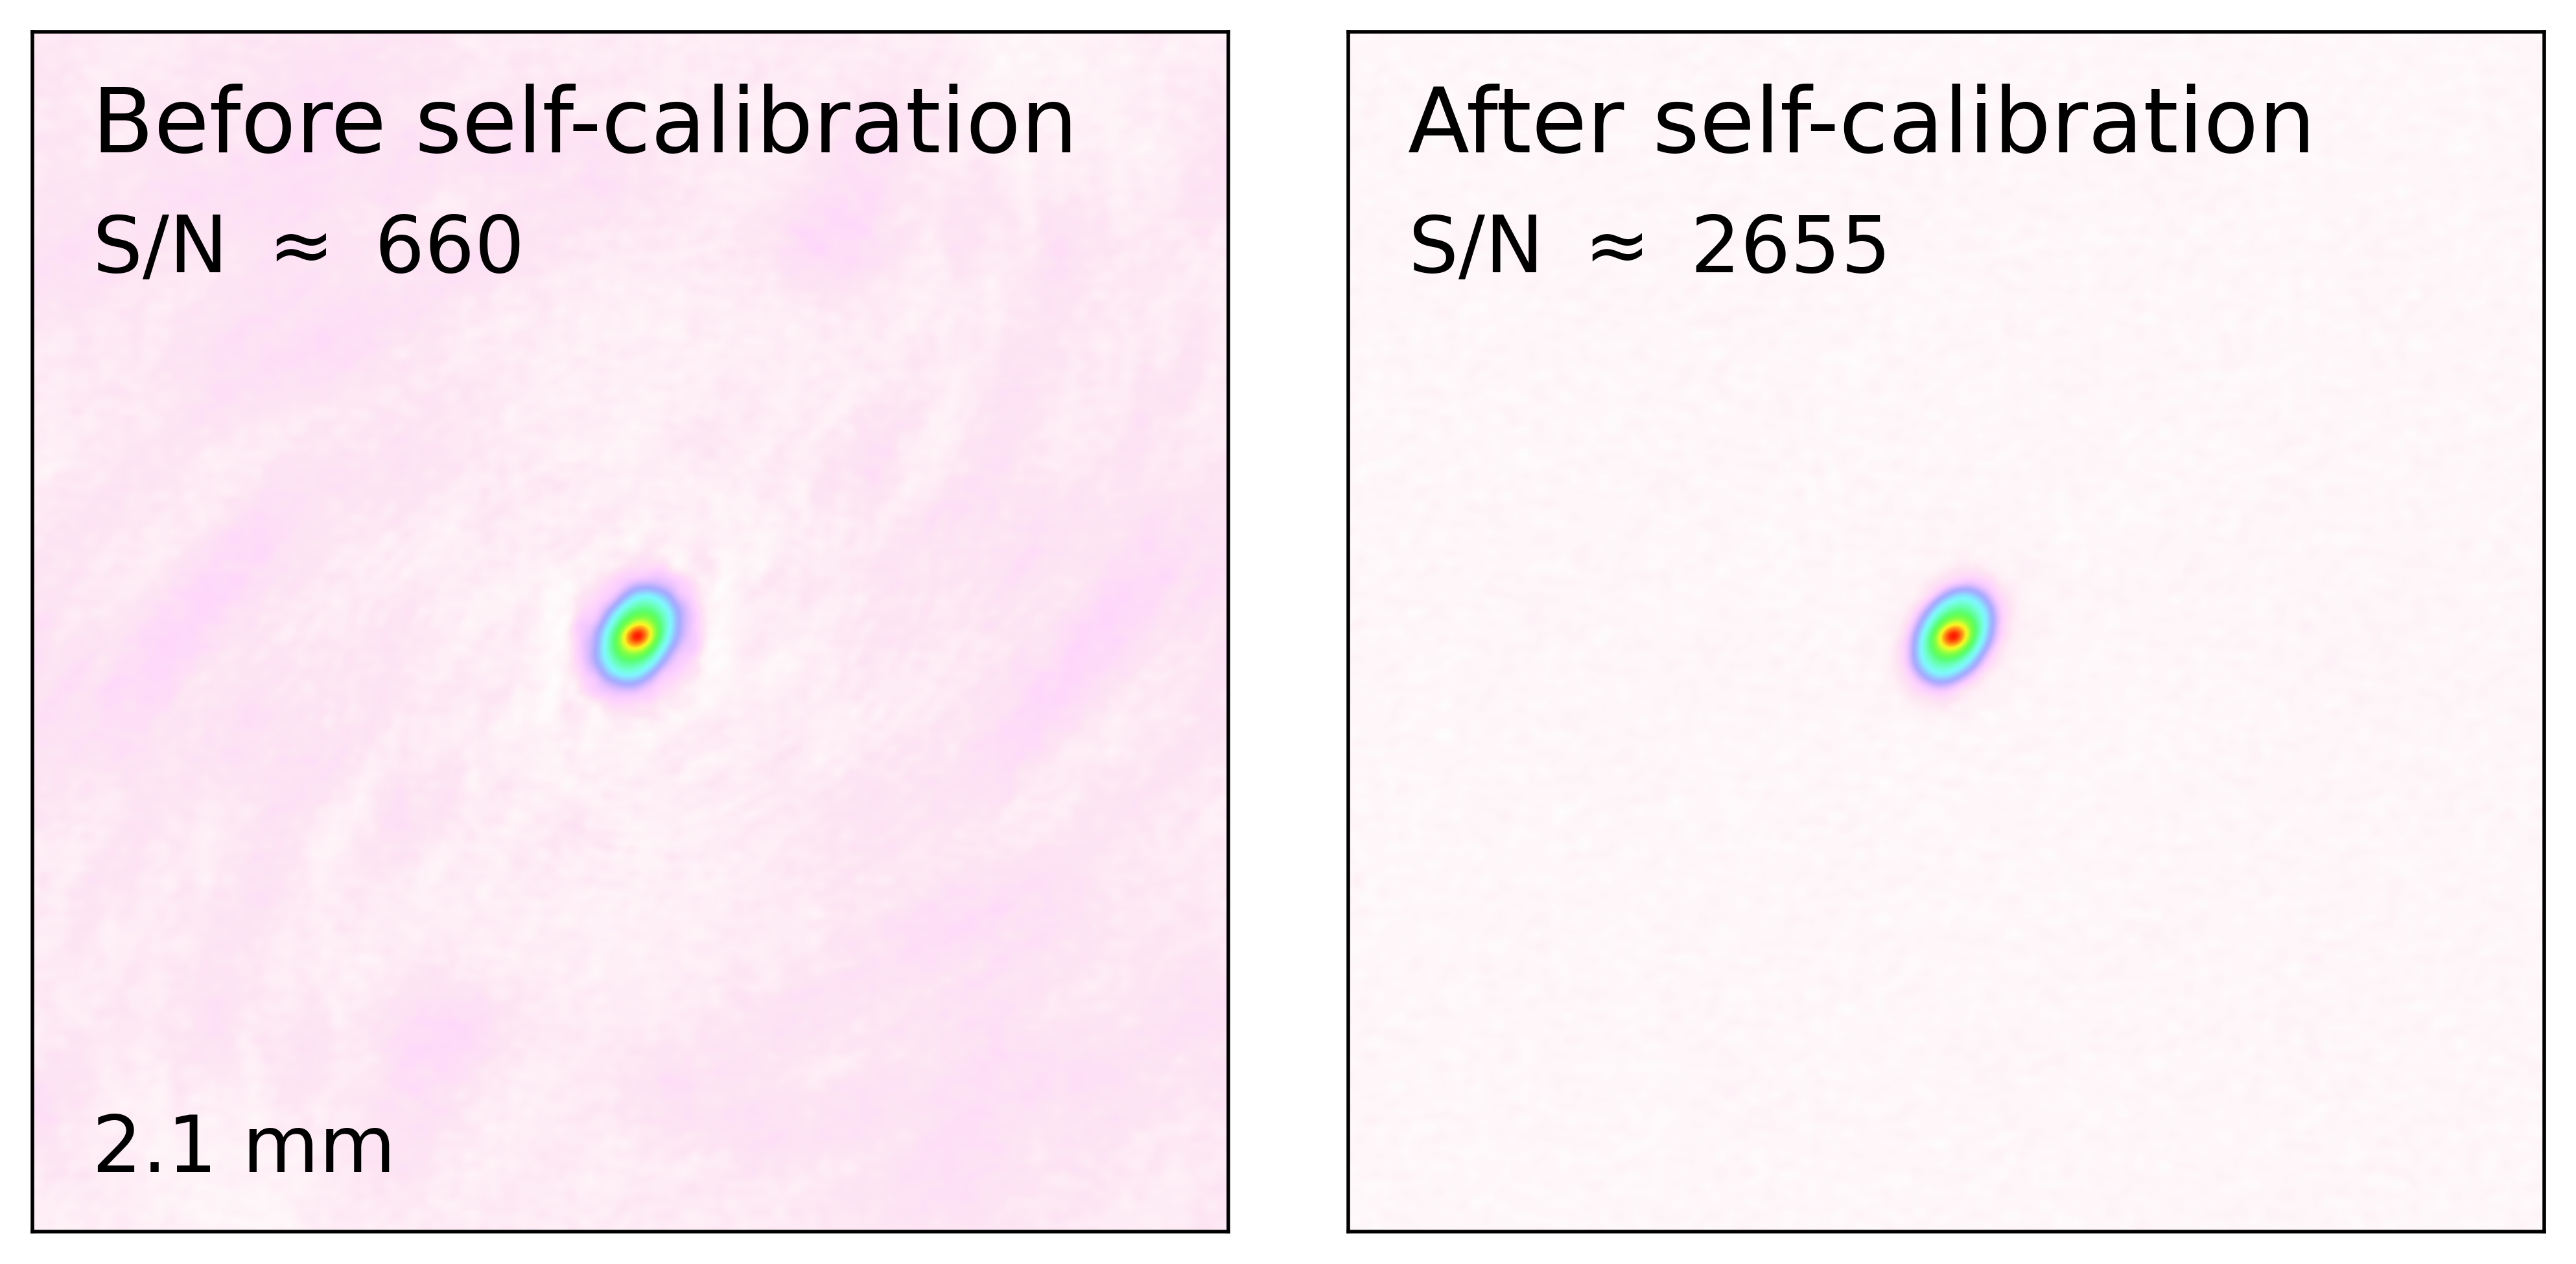
\includegraphics[width=0.99\textwidth]{WRITEUP_AND_IMAGES/IMAGES/WRITEUP/BeforeAndAfterClean.png}
  \caption[Images before and after self-calibration.]{Images before (left) and after (right) self-calibration at \bfourNS. The images demonstrate how background noise is reduced during the self-calibration process, improving the peak \SNRns.}
  \label{fig: BeforeAndAfterClean}
\end{figure}



Additionally, the \SQ and \SU data were cleaned using \texttt{tclean}, using the final mask from the final \texttt{tclean} step at its respective wavelength. The same Briggs \texttt{robust} value used for \SI was used for \SQ and $U$, with \texttt{nterms = 1}.  
% Checked this for all bands
% \sudo{Checked this for Band 4 and 7. Can check 5 and 7 when I can access my data again. "Please do" - Sarah}










Table \ref{tab: source_info} lists the resulting image resolution after self-calibration, including the synthesized beam parameters and clean details. The table also includes the disk centre position in Right Ascension (RA) and Declination (Dec), as well as the disk position angle found by fitting a Gaussian to the disk using \texttt{imfit} in CASA. The image sensitivities are also provided and were determined using the method described in Chapter \ref{sec: stokes_errors}. 


\begin{table}[h!]
\centering
\caption[Summary of the properties of the cleaned images of IRS 63.]{Summary of the properties of the cleaned images of IRS 63 at each wavelength. }
\begin{tabular}{lcccc}
\toprule
\textbf{Property} & \textbf{\bandfourmm} & \textbf{\bandfivemm } & \textbf{\bandsixmm } & \textbf{\bandsevenmm} \\
\midrule


R.A. (h, m, s) 
& 16:31:35.656 
& 16:31:35.656 % Updated July 22
& 16:31:35.657  
& 16:31:35.656 \\

Decl. ($^\circ$, $'$, $''$) 
& -24:01:29.992 
& -24:01:30.086 % Updated July 22
& -24:01:29.935 
& -24:01:30.089 \\


Beam ($''\times''$) 
& 0.18 $\times$ 0.13 
& 0.23 $\times$ 0.18 
& 0.27 $\times$ 0.20 
& 0.28 $\times$ 0.17 \\



Beam PA ($^\circ$) 
& -81.0 
& -97
& -68.6
& -81.2 \\

% Deconvolved from beam
Disk PA ($^\circ$) 
& 145.9 
& 148.4 % This was checked on July 22
& 148.0 
& 139.7 \\

\texttt{nterms}
& 2
& 1
& 1
& 2 \\

\texttt{robust}
& 0.5
& -1
& 0.5 
& 0.5 \\



\SIerr  (\ujybeamNS)
& 14
& 42
& 71
& 35 \\

\SQerr (\ujybeamNS)
& 9.7
& 13 % 41
& 27
& 26 \\

\SUerr (\ujybeamNS)
& 10
& 15 % 41
& 27
& 24 \\




\bottomrule
\end{tabular}
\begin{tablenotes}
% \footnotesize
\item \textbf{Note:} \SIerrNS, \SQerrNS, and \SUerr are representative of the sensitivity at the phase center for each wavelength. \note{I accidentally then changed Ierr to 13 and kept Qerr as 41. Ierr is 42 and Qerr is 13. }
\end{tablenotes}
\label{tab: source_info}
\end{table}




% -------------------------------------------------------------

% -------------------------------------------------------------
\section{Debias Correction}
\label{sec: debias_correction}
% -------------------------------------------------------------

The observed polarized intensity, \POLIobsNS, is calculated from \SQ ($Q$) and \SU ($U$) using the equation: 
\begin{equation}
    \POLIobsEQ = \sqrt{Q^2 + U^2}.
    \label{eq: POLI}
\end{equation}
\noindent Since \SQ and $U$ are squared, the equation always yields a positive value. This introduces a positive bias when either \SQ or $U$ are dominated by noise, since noise can cause non-zero values even when there is no polarized emission. To account for this bias, a debiased polarized intensity is calculated. 
% noise gives us Q and U not equal to 0 even when it should be 0, more noise -> higher POLI value



The polarized intensity was debiased using the method explained in \cite{sadavoy_dust_2019}, originally from \cite{HullDebias}. Table \ref{tab: stokes_polar_variables} summarizes the variables used in these equations and throughout the remainder of this section. This method calculates the debiased polarized intensity, \POLIns, given a corresponding error of \POLIerrNS, with the equation:

\begin{equation}
    \text{PDF}(\POLIeq|\POLIobsEQ, \POLIerrEQ)=\frac{\POLIobsEQ}{\POLIerrEQ^2} I_0(x)\exp\left[-\frac{(\POLIobsEQ^2 + \POLIeq^2)}{2\POLIerrEQ^2}{}\right],
    \label{eq: debias}
\end{equation}
\noindent where PDF is the probability density function. Here, $I_0(x)$ is the Bessel function for the Bessel parameter $x = \POLIobsEQ \POLIeq/\POLIerrEQ^2$. The most likely \POLI corresponds to the peak of the PDF in Equation \ref{eq: debias}. The debiased value is calculated by minimizing the negative value of the PDF in Equation \ref{eq: debias} using \texttt{scipy.optimize.minimize\_scalar}. 



\begin{table}[h!]
\centering
\caption[Summary of Stokes and polarization parameterss.]{Summary of Stokes and polarization parameters, their associated error symbols, and units.  \question{Trying to show I am reporting Stokes parameters in mJy/beam and units in $\mu$Jy/beam, better way than: \mjybeam / \ujybeam}}
\begin{tabular}{llll}
\toprule
\textbf{Parameter} & \textbf{Symbol} & \textbf{Error} & \textbf{Units}  \\
\midrule


\SI
& I
& \SIerr
& \mjybeam / \ujybeam\\

\SQ
& Q
& \SQerr
& \mjybeam  / \ujybeam\\

\SU
& U
& \SUerr
& \mjybeam  / \ujybeam\\



% Observed (Biased) Polarized Intensity
% & \POLIobs
% & N/A
% & \mjybeam\\


Debiased Polarized Intensity
& \POLI
& \POLIerr
& \mjybeam\\

Debiased Polarization Fraction 
& \POLF
& \POLFerr
& percent (\%)\\


Polarization Angle 
& $\theta$
& \PAerr
& radians \\





\bottomrule
\end{tabular}
\label{tab: stokes_polar_variables}
\end{table}








Only the pixels with a low to moderate S/N, below 9, were debiased with the method described above. The pixels with S/N$>9$ do not need to be treated the same way because their emission is much stronger than the noise. These pixels are debiased using the standard maximum likelihood calculation method from \cite{VaillancourtDebias}:
\begin{equation}
   \POLIbrightEQ = \sqrt{Q^2 + U^2 -\POLIerrEQ^2}.
\end{equation}


\noindent The error in polarized density is defined following \citep{CoudeEquations} as:

\begin{equation}
    \POLIerrEQ = 
    \left[ 
    \frac{(Q\SQerrEQ)^2 + (U\SUerrEQ)^2}{Q^2 + U^2} \right]^{1/2}.
    \label{eq: POLI_error}
\end{equation}

% -------------------------------------------------------------






% -------------------------------------------------------------
\section{Additional Polarization Quantities \& Errors}
% -------------------------------------------------------------


% ---------------------------------------------
\subsection{Errors for Stokes Parameters}
\label{sec: stokes_errors}

For the data calibrated in this project (\bfourNS, \bfiveNS, \bsevenNS), the errors for \SIns, \SQ and \SU were estimated by averaging the standard deviation in four different regions far from the bright source at the centre. The standard deviations were measured without applying a primary beam correction. This average value was applied as a constant error at every pixel in the respective error maps. The source is small and located at the phase centre of the observations where the primary beam is approximately flat. Therefore, adopting a constant error across the disk is reasonable. Table \ref{tab: source_info} gives the errors at each wavelength. The errors for the \bsix data were estimated using the same method from \cite{sadavoy_dust_2019}. 

% ---------------------------------------------
\subsection{Polarization Fraction and Angle}

The following equations in this Chapter are from \cite{CoudeEquations}, unless specified otherwise. 

Using the debiased polarized intensity, the debiased polarization fraction can be calculated by:
\begin{equation}
    \POLFeq = \POLIeq/I,
    \label{eq: POLF}
\end{equation}
\noindent where $I$ is \SI intensity. The uncertainty on polarization fraction is:

\begin{equation}
    \POLFerrEQ = \POLFeq \left[\left(\frac{\POLIerrEQ}{\POLIeq}\right)^2 + \left(\frac{\SIerrEQ}{I}\right)^2\right]^{1/2}.
     \label{eq: POLF_error}
\end{equation}
   


The polarization position angle, $\theta$ is calculated as: 
\begin{equation}
\theta = \half \tan ^{-1} \frac{U}{Q},
    \label{eq: PA}
\end{equation}
\noindent where $\theta$ has units of radians, and an uncertainty calculated by:

\begin{equation}
    \PAerrEQ = \frac{1}{2} 
    \frac{\sqrt{(U\SQerrEQ)^2 + (Q\SUerrEQ)^2}}{Q^2 + U^2}.
    \label{eq: PA_error}
\end{equation}
 

\noindent When measuring the angles, the zero-degree position is defined as North, with the polarization angle increasing counterclockwise from North to East. The coordinate system was previously shown in see Figure \ref{fig: LinearPol}. 

% ---------------------------------------------








% -------------------------------------------------------------

